\documentclass{article}
\usepackage{amsmath, amssymb}
\usepackage{tikz}
\usepackage[most]{tcolorbox}
\usetikzlibrary{positioning, arrows.meta, shapes.multipart, calc}

\definecolor{heisblue}{RGB}{40,90,140}
\definecolor{arithgreen}{RGB}{60,120,60}
\definecolor{centerpurple}{RGB}{110,80,150}

\tikzset{
box/.style={
    draw,
    rounded corners,
    thick,
    align=left,
    inner sep=8pt,
    font=\small,
    text width=6cm
},
title/.style={
    font=\bfseries
}
}

\begin{document}

\begin{center}
{\LARGE \textbf{H3 (Cohomological Alignment): Arithmetic = Heisenberg}}
\end{center}

\vspace{1em}

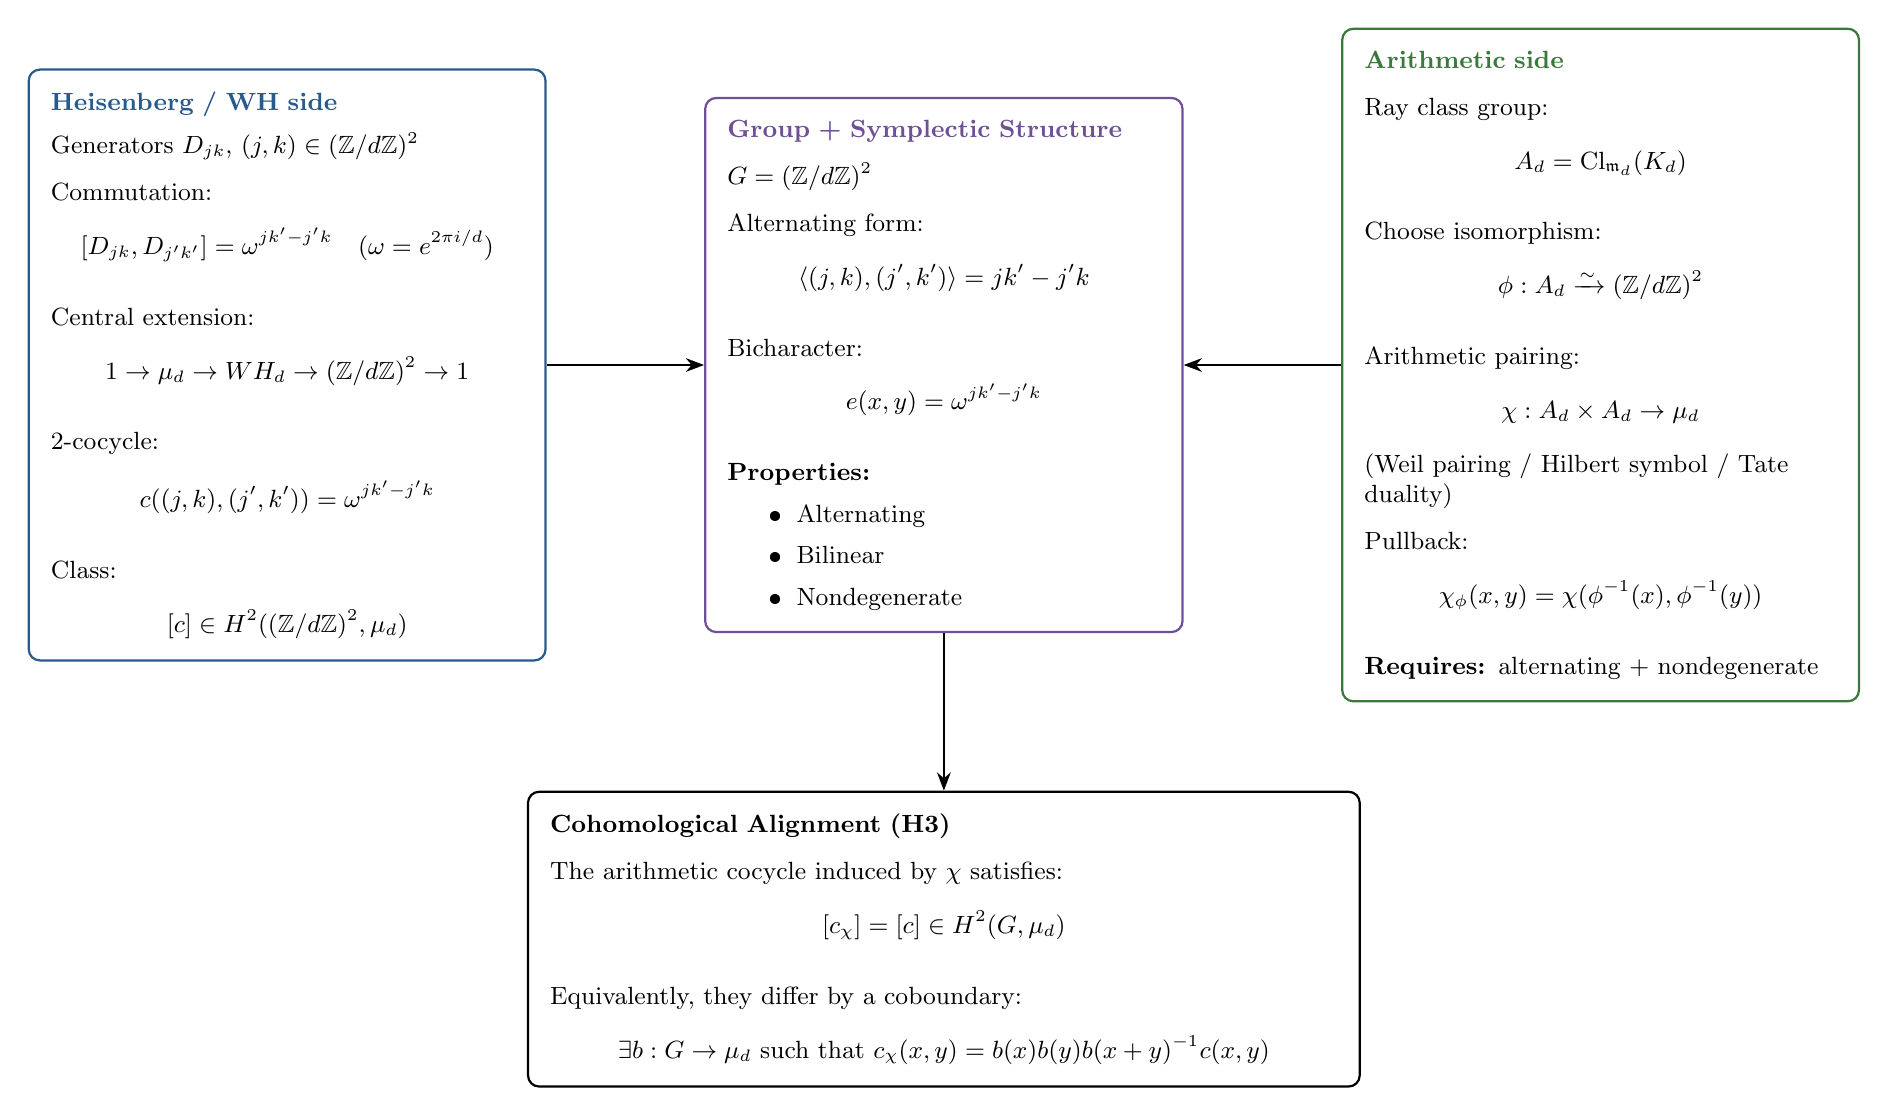
\begin{tikzpicture}[
    node distance=1.8cm and 2cm,
    >=Stealth
]

% LEFT: HEISENBERG
\node[box, draw=heisblue] (heis) {
\textbf{\color{heisblue}Heisenberg / WH side}

\vspace{0.5em}

Generators $D_{jk}$, $(j,k)\in (\mathbb{Z}/d\mathbb{Z})^2$

\medskip

Commutation:
\[
[D_{jk}, D_{j'k'}] = \omega^{jk'-j'k}
\quad (\omega = e^{2\pi i/d})
\]

\medskip

Central extension:
\[
1 \to \mu_d \to WH_d \to (\mathbb{Z}/d\mathbb{Z})^2 \to 1
\]

\medskip

2-cocycle:
\[
c((j,k),(j',k')) = \omega^{jk'-j'k}
\]

\medskip

Class:
\[
[c] \in H^2((\mathbb{Z}/d\mathbb{Z})^2, \mu_d)
\]
};

% CENTER: GROUP STRUCTURE
\node[box, draw=centerpurple, right=of heis, text width=5.5cm] (center) {
\textbf{\color{centerpurple}Group + Symplectic Structure}

\medskip

$G = (\mathbb{Z}/d\mathbb{Z})^2$

\medskip

Alternating form:
\[
\langle (j,k),(j',k') \rangle = jk' - j'k
\]

\medskip

Bicharacter:
\[
e(x,y) = \omega^{jk'-j'k}
\]

\medskip

\textbf{Properties:}
\begin{itemize}
\item Alternating
\item Bilinear
\item Nondegenerate
\end{itemize}
};

% RIGHT: ARITHMETIC
\node[box, draw=arithgreen, right=of center] (arith) {
\textbf{\color{arithgreen}Arithmetic side}

\medskip

Ray class group:
\[
A_d = \mathrm{Cl}_{\mathfrak{m}_d}(K_d)
\]

\medskip

Choose isomorphism:
\[
\phi: A_d \xrightarrow{\sim} (\mathbb{Z}/d\mathbb{Z})^2
\]

\medskip

Arithmetic pairing:
\[
\chi: A_d \times A_d \to \mu_d
\]

(Weil pairing / Hilbert symbol / Tate duality)

\medskip

Pullback:
\[
\chi_\phi(x,y) = \chi(\phi^{-1}(x), \phi^{-1}(y))
\]

\medskip

\textbf{Requires:}
alternating + nondegenerate
};

% BOTTOM ALIGNMENT
\node[box, draw=black, below=2cm of center, text width=10cm] (align) {
\textbf{Cohomological Alignment (H3)}

\medskip

The arithmetic cocycle induced by $\chi$ satisfies:
\[
[c_\chi] = [c] \in H^2(G, \mu_d)
\]

\medskip

Equivalently, they differ by a coboundary:
\[
\exists b:G \to \mu_d \text{ such that }
c_\chi(x,y) = b(x)b(y)b(x+y)^{-1} c(x,y)
\]
};

% ARROWS
\draw[->, thick] (heis) -- (center);
\draw[->, thick] (arith) -- (center);
\draw[->, thick] (center) -- (align);

\end{tikzpicture}

\vspace{1em}

\begin{tcolorbox}[colback=red!5, colframe=red!60!black, title=Failure Modes]
\textbf{Not alternating:} introduces symmetric component $\Rightarrow$ wrong cohomology class.

\medskip

\textbf{Degenerate:} factors through quotient $\Rightarrow$ cannot represent Heisenberg class.
\end{tcolorbox}

\end{document}